\section{Constraint Processing}
\label{s:constraintProcessing}
\chapterquote{Alle beperking maakt gelukkig.}{Arthur Schopenhauer, Duits filosoof (1788-1860)}
Een alternatief voor zoekalgoritmen bij het oplossen van zoekproblemen, is \termen{Constraint Processing}. Zoals de naam al doet vermoeden kan constraint processing alleen maar een bepaald type zoekproblemen oplossen: \termen{Constraint Problems}.
\subsection{Wat zijn Constraint Problems?}
Constraint problemen zijn problemen die bestaan uit:
\begin{itemize}
 \item een set variabelen: $z_1,z_2,\ldots,z_n$
 \item een eindig domein per variabele: $\mathfunc{dom}{z_i}=d_i=\left\{a_{i\,1},a_{i\,2},\ldots,a_{i\,n_i}\right\}$
 \item een set constraints ($c:d_i\times d_j\times\ldots\times d_l\rightarrow\Bb$): een functie die waar teruggeeft indien aan een bepaalde eis gerelateerd aan de variabelen van de constraint voldaan wordt, anders vals. Constraints worden opgesplitst worden in drie types:
\begin{itemize}
\item \termen{Unaire constraints}: iedere variabele $z_i$ heeft een constraint $c\left(z_i\right)$
\item \termen{Binaire constraints}: voor iedere twee variabelen $z_i$ en $z_j$ met $i<j$: $c\left(z_i,z_j\right)$
\item Optioneel \termen{Meervoudige constraints}: $c\left(z_i,z_j,\ldots,z_l\right)$, deze constraints worden echter buiten beschouwing gelaten en zijn eerder uitzonderlijk
\end{itemize}
\end{itemize}
Formeel stelt het probleem concrete waarden voor de variabelen te vinden die een element zijn van hun respectievelijk domein, en daarenboven zo dat aan alle constraint voldaan wordt. Dit kan uiteraard gedaan worden met de reeds behandelde zoekalgoritmen. Voor dergelijke problemen bestaan er echter effici\"entere oplossingsmethodes.
\subsection{Leidend Voorbeeld: 4-Teachers}
\begin{leftbar}
We introduceren een fictief probleem (omdat dit probleem relatief eenvoudig is, en vele concepten illustreert). We stellen 4 professoren ($A$,$B$,$C$,$D$). En 5 lokalen. Elke professor dient een bepaalde les te geven. Uiteraard kunnen er geen twee lessen in eenzelfde lokaal plaatsvinden. Daarnaast blijken de professoren nog enkele voorkeuren te hebben:
\begin{enumerate}
 \item professor $A$ wil geen les geven in lokaal 3 en wil hoogstens 2 lokalen verwijdert zijn van prof. $B$. Het lokaalnummer dient minstens twee groter te zijn dan dat van professor $D$.
 \item professor $B$ wil geen les geven in lokaal 5. En in een lokaal met een nummer dat minstens 2 groter is dan dat van professor $C$.
 \item professor $C$ wil alleen les geven in lokalen kleiner of gelijk aan 3. Met minstens \'e\'en lokaal tussen professor $A$.
 \item professor $D$ wil les geven in een lokaal dat exact 2 kleiner is dan het lokaal van professor $B$.
\end{enumerate}
De enige oplossing voor dit probleem is: $\left(A,B,C,D\right)=\left(5,4,1,2\right)$. Formeel drukken we deze situatie nu als volgt uit: We beschikken over vier variabelen $A$, $B$, $C$ en $D$. Elke variabele heeft hetzelfde domein, $d_A=d_B=d_C=d_D=\left\{1,2,3,4,5\right\}$. Als unaire constraints hebben we:
\begin{equation}
\left\{\begin{array}{l}
c(A)\leftrightarrow A\neq 3\\
c(B)\leftrightarrow B\neq 5\\
c(C)\leftrightarrow C\leq 3\\
c(D)\leftrightarrow \true
\end{array}\right.
\end{equation}
Als binaire constraint beschikken we over:
\begin{equation}
\left\{\begin{array}{l}
c(A,B)\leftrightarrow\left|A-B\right|\in\left\{1,2\right\}\\
c(A,C)\leftrightarrow\left|A-C\right|>1\\
c(A,D)\leftrightarrow D<A-1\\
c(B,C)\leftrightarrow C<B-1\\
c(B,D)\leftrightarrow D=B-2\\
c(C,D)\leftrightarrow C\neq D
\end{array}\right.
\end{equation}
\end{leftbar}
\subsection{Node-consistency}
Unaire constraints zijn slechts gerelateerd aan 1 variabele, hierdoor kunnen we deze al doen kloppen nog voor we een van de oplossingsmethodes gebruiken. Hiervoor gebruiken we \termen{Node-consistency}, ook wel \termen{1-consistency} genoemd. Deze techniek reduceert eenvoudigweg het domein van de variabele tot enkel die waarden waarvoor de constraint klopt. Voor iedere variabele $z_i$ genereren we dus een nieuw domein $d_i'$ met:
\begin{equation}
d_i'=\left\{a|a\in d_i\wedge c\left(z_i=a\right)\right\}
\end{equation}
\begin{leftbar}
Toegepast op ons voorbeeld genereren we dus een nieuw domein voor iedere variable met:
\begin{equation}
\begin{array}{lclcl}
d_A=\left\{1,2,3,4,5\right\}&\wedge&c\left(A\right)\leftrightarrow A\neq 3&\Rightarrow&d_A'=\left\{1,2,4,5\right\}\\
d_B=\left\{1,2,3,4,5\right\}&\wedge&c\left(B\right)\leftrightarrow B\neq 5&\Rightarrow&d_B'=\left\{1,2,3,4\right\}\\
d_C=\left\{1,2,3,4,5\right\}&\wedge&c\left(C\right)\leftrightarrow C\leq 3&\Rightarrow&d_C'=\left\{1,2,3\right\}\\
d_D=\left\{1,2,3,4,5\right\}&\wedge&c\left(D\right)\leftrightarrow\true&\Rightarrow&d_D'=\left\{1,2,3,4,5\right\}
\end{array}
\end{equation}
\end{leftbar}
\subsection{Visuele voorstelling van het probleem}
We kunnen een dergelijk probleem visueel voorstellen: door middel van een \termen{OR-tree} of met een \termen{Constraint Network}. Deze twee voorstellen vertegenwoordigen bovendien twee totaal verschillende strategie\"en om een dergelijk probleem op te lossen. Voorbeelden van de twee voorstellingen zijn respectievelijk te zien op figuren \ref{fig:fourTeachersORTree} en \ref{fig:fourTeachersConstraintNetwork}.
\subsubsection{De OR-tree voorstelling}
Bij een OR-tree selecteren we een orde in de variabelen, en vervolgens wijzen we aan de hand van die orde een bepaalde laag $i$ van de boom toe aan variabele $z_i$. Onder iedere knoop die in de laag erboven $i-1$ aan alle constraints $\forall j<i-1: c\left(z_j,z_{i-1}\right)$ voldoet, genereren we vervolgens knopen, waarbij elke knoop \'e\'en van de domeinwaarden van $z_i$ draagt. Daaronder testen we vervolgens de constraints op de dan reeds ingevulde waarden: $\forall j<i: c\left(z_j,z_{i}\right)$. We passen dit proces iteratief toe in de diepte van de boom.
\paragraph{}
Het zoeken naar een oplossing met behulp van een dergelijke boom, werkt met ongeveer dezelfde principes als de zoekalgoritmen beschreven in sectie \ref{s:searchMethods}. We kunnen echter enkele optimalisaties toepassen door het kiezen van goede \termen{backtrack}-algoritmen. Dit zijn algoritmen die geactiveerd worden op het moment dat we in een knoop zitten waar we geen verdere onderliggende knopen meer kunnen evalueren en dus een niveau terug moeten keren, deze technieken worden besproken in subsectie \ref{ss:backtrackingsAlgorithms}.
\begin{leftbar}
Een uitgewerkte OR-tree voor het 4-Teachers probleem staat op figuur \ref{fig:fourTeachersORTree}.
\end{leftbar}
\begin{figure}[htb]
\centering
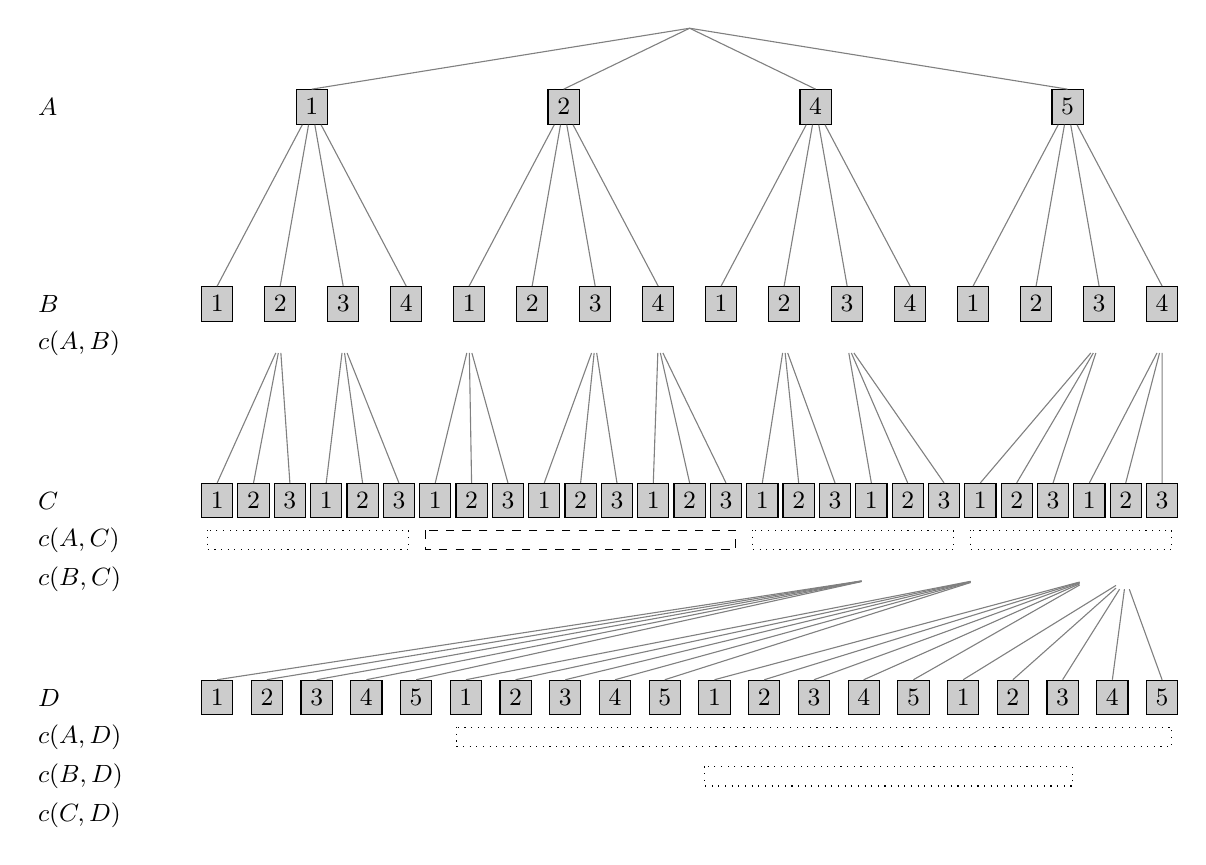
\begin{tikzpicture}[vari/.style={fill=black!20,rectangle,draw=black}]
\def\da{3.2};
\def\db{0.8};
\def\dc{0.461538};
\def\dd{0.631578947};
\def\dy{-2.5};
\foreach\y/\yt in {0/A,1/B,2/C,3/D} {
  \draw (-0.4,\dy*\y) node[anchor=west] {\small{$\yt$}};
}
\foreach\x/\y/\xt/\yt in {1/2/A/B,1/3/A/C,1/4/A/D,2/3/B/C,2/4/B/D,3/4/C/D} {
  \draw (-0.4,\dy*\y-0.5*\x-\dy) node[anchor=west] {\small{$c(\xt,\yt)$}};
}
\coordinate (S0) at (\da*2.5,1);
\foreach\x/\xt in {1/1,2/2,3/4,4/5} {
  \node[vari] (SA) at (\da*\x,0) {\small{$\xt$}};
  \draw[thin,gray] (S0) -- (SA.north);
  \foreach\y in {1,2,3,4} {
    \node[vari] (SB) at (\da*\x+\db*\y-\db*2.5,\dy) {\small{$\y$}};
    \draw[thin,gray] (SA) -- (SB.north);
  }
}

\foreach\x in {1,4,6,9,12,13,14} {
  \draw (\da+\db*\x-\db*2.5,\dy-0.5) node {\small{$\XBox$}};
}
\foreach\x in {2,3,5,7,8,10,11,15,16} {
  \node (Sv\x) at (\da+\db*\x-\db*2.5,\dy-0.5) {\small{$\CheckedBox$}};
}
\foreach\x/\xr in {1/2,2/3,3/5,4/7,5/8,6/10,7/11,8/15,9/16} {
  \foreach\y in {1,2,3} {
    \node [vari] (SC) at (\da+3*\dc*\x+\dc*\y-4*\dc-\db*1.5,2*\dy) {\small{$\y$}};
    \draw[thin,gray] (Sv\xr) -- (SC.north);
  }
}
\foreach\x in {1,2,4,5,7,8,9,10,11,12,13,14,15,18,21} {
  \node (Sv\x) at (\da+\dc*\x-\dc-\db*1.5,2*\dy-0.5) {\small{$\XBox$}};
}
\foreach\x in {3,6,16,17,19,20,22,23,24,25,26,27} {
  \node (Sv\x) at (\da+\dc*\x-\dc-\db*1.5,2*\dy-0.5) {\small{$\CheckedBox$}};
}
\draw[dotted] (Sv1.north west) rectangle (Sv6.south east);
\draw[dashed] (Sv7.north west) rectangle (Sv15.south east);
\draw[dotted] (Sv16.north west) rectangle (Sv21.south east);
\draw[dotted] (Sv22.north west) rectangle (Sv27.south east);
\foreach\x in {6,17,24,3,16,20,23,27} {
  \node (Sv\x) at (\da+\dc*\x-\dc-\db*1.5,2*\dy-1) {\small{$\XBox$}};
}
\foreach\x in {19,22,25,26} {
  \node (Sv\x) at (\da+\dc*\x-\dc-\db*1.5,2*\dy-1) {\small{$\CheckedBox$}};
}
\foreach\x/\xr in {1/19,2/22,3/25,4/26} {
  \foreach\y in {1,2,3,4,5} {
    \node [vari] (SD) at (\da+5*\dd*\x+\dd*\y-6*\dd-\db*1.5,3*\dy) {\small{$\y$}};
    \draw[thin,gray] (Sv\xr) -- (SD.north);
  }
}
\foreach\x in {3,4,5,9,10,14,15,19,20} {
  \node (Sv\x) at (\da+\dd*\x-\dd-\db*1.5,3*\dy-0.5) {\small{$\XBox$}};;
}
\foreach\x in {1,2,6,7,8,11,12,13,16,17,18} {
  \node (Sv\x) at (\da+\dd*\x-\dd-\db*1.5,3*\dy-0.5) {\small{$\CheckedBox$}};
}
\draw[dotted] (Sv6.north west) rectangle (Sv20.south east);
\foreach\x in {2,7,8,11,13,16,18} {
  \node (Sv\x) at (\da+\dd*\x-\dd-\db*1.5,3*\dy-1) {\small{$\XBox$}};;
}
\foreach\x in {1,6,12,17} {
  \node (Sv\x) at (\da+\dd*\x-\dd-\db*1.5,3*\dy-1) {\small{$\CheckedBox$}};;
}
\draw[dotted] (Sv11.north west) rectangle (Sv18.south east);
\foreach\x in {1,6,17} {
  \node (Sv\x) at (\da+\dd*\x-\dd-\db*1.5,3*\dy-1.5) {\small{$\XBox$}};
}
\node (Sv) at (\da+11*\dd-\db*1.5,3*\dy-1.5) {\small{$\CheckedBox$}};
\end{tikzpicture}
\caption{OR-tree van het 4-teachers probleem.}
\label{fig:fourTeachersORTree}
\end{figure}
\subsubsection{Het Constraint Network}
Bij een constraint network stellen we het probleem voor als een grafe. Hierbij vertegenwoordigt iedere knoop een bepaalde variabele. Bogen tussen verschillende punten, vertegenwoordigen dan weer de constraint tussen de twee variabelen van die punten. Verder kennen we ook een verzameling mogelijk waarden toe aan een punt, initieel is deze gelijk aan het domein van deze variabele. Vervolgens overlopen we iedere constraint. Indien bepaalde elementen in het domein van een variabele niet mogelijk zijn, worden deze uit het domein verwijdert. Dit proces heet \termen{relaxation} of \termen{relaxatie} en wordt verder beschreven in subsectie \ref{ss:relaxationAndHybridConstraintProcessing}. Het verwijderen van enkele variabelen kan een kettingreactie tot gevolg hebben. Dit resulteert in het beste geval tot \'e\'en element per variabele. Meestal loopt het echter niet zo'n vaart, en wordt het probleem opgelost met een backtrackingsalgoritme die met de gereduceerde domeinen het probleem sneller oplost.
\begin{leftbar}
Indien we dit toepassen op de het 4-Teachers probleem bekomen we een Constraint Network zoals beschreven op figuur \ref{fig:fourTeachersConstraintNetwork}.
\end{leftbar}
\begin{figure}[htb]
\centering
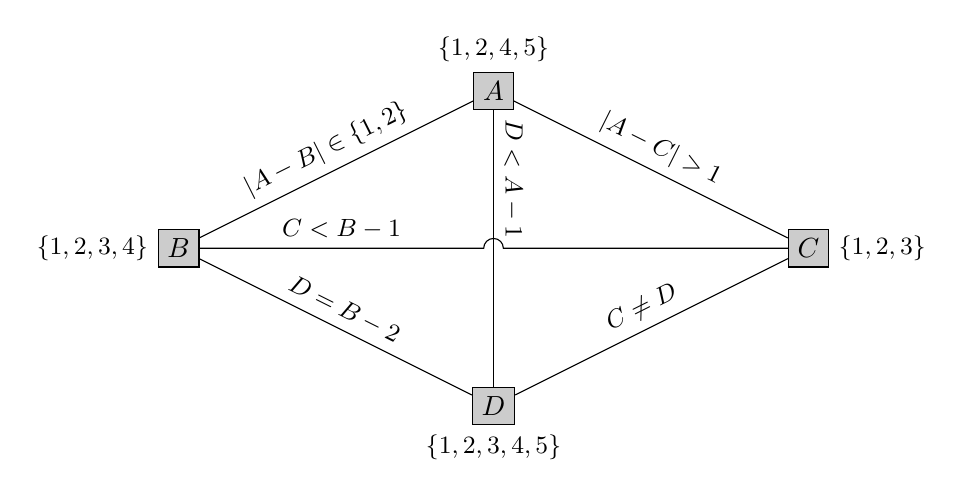
\begin{tikzpicture}[vari/.style={fill=black!20,rectangle,draw=black}]
\def\dx{4};
\def\dy{2};
\def\r{0.125};
\node[vari] (A) at (0,\dy) {$A$};
\node[vari] (B) at (-\dx,0) {$B$};
\node[vari] (C) at (\dx,0) {$C$};
\node[vari] (D) at (0,-\dy) {$D$};
\node[anchor=south] (DA) at (A.north) {\small{$\left\{1,2,4,5\right\}$}};
\node[anchor=east] (DB) at (B.west) {\small{$\left\{1,2,3,4\right\}$}};
\node[anchor=west] (DC) at (C.east) {\small{$\left\{1,2,3\right\}$}};
\node[anchor=north] (DD) at (D.south) {\small{$\left\{1,2,3,4,5\right\}$}};
\draw (A) to node[midway,sloped,above]{\small{$\left|A-B\right|\in\left\{1,2\right\}$}} (B);
\draw (A) to node[midway,sloped,above]{\small{$\left|A-C\right|>1$}} (C);
\draw (A) to node[midway,sloped,above]{\small{$D<A-1$}} (0,0) -- (D);
\draw (B) to node[midway,sloped,above]{\small{$C<B-1$}} (-\r,0) arc (180:0:\r) -- (C);
\draw (B) to node[midway,sloped,above]{\small{$D=B-2$}} (D);
\draw (C) to node[midway,sloped,above]{\small{$C\neq D$}} (D);
\end{tikzpicture}
\caption{Constraint Network van het 4-teachers probleem.}
\label{fig:fourTeachersConstraintNetwork}
\end{figure}
\subsection{Backtrack algoritmen}
\label{ss:backtrackingsAlgorithms}
Indien we het probleem oplossen met de OR-tree benadering, komen we vaak situaties tegen waarbij we geen kinderen van een bepaalde knoop meer kunnen evalueren. Dit komt bijvoorbeeld omdat alle kinderen ge\"evalueerd zijn. In zo'n geval is het de bedoeling dat we \'e\'en of meer niveaus terugspringen. Hiervoor bestaan verschillende implementaties die vooral tot doel hebben om nutteloos op constraints te controleren te vermijden. Deze worden beschreven in subsubsecties \ref{sss:chronolgicalBacktracking} tot \ref{sss:dynamicSearchRearrangement}.
\subsubsection{Chronological Backtracking}
\label{sss:chronolgicalBacktracking}
\termen{Chronological Backtracking} is veruit het eenvoudigste algoritme. Indien we dit algoritme toepassen bekomen we niets minder dan diepte-eerst zoeken toegepast op de OR-boom. Met andere woorden hierbij wordt eenvoudigweg naar de ouder teruggekeerd, en de knoop rechts van de huidige knoop wordt vervolgens ge\"evalueerd. Indien ook in de ouder geen knoop meer te evalueren is, treed er een recursief effect op, waarbij we telkens een niveau hoger gaan tot er uiteindelijk weer een volgende knoop beschikbaar is.
\begin{algorithm}[htb]
\caption{$\mathcommand{chronologicalBacktracking}{\depth}$}
\label{alg:chronologicalBacktracking}
\begin{algorithmic}[1]
\FOR{$k=1$ to $n_{\depth}$}
\STATE\COMMENT{Iteratie over alle knopen op niveau $\depth$}
\STATE$z_{\depth}\leftarrow a_{\depth\,k}$\COMMENT{Geef $z_{\depth}$ een concrete waarde}
\STATE$b\leftarrow\true$
\STATE\COMMENT{Controleer alle constraints met $z_i$}
\FOR{$j=1$ to $\depth-1$}
\STATE $b\leftarrow b\wedge c\left(z_j,z_i\right)$
\ENDFOR
\IF{$b$}
\STATE\COMMENT{Alle constraints kloppen}
\IF{$\depth=n$}
\STATE\COMMENT{Laatste niveau bereikt, oplossing gevonden!}
\RETURN$\left(z_1,z_2,\ldots,z_n\right)$
\ELSE
\STATE\COMMENT{Naar het volgende niveau}
\STATE$\mathcommand{chronologicalBacktracking}{\depth+1}$
\ENDIF
\ENDIF
\ENDFOR
\end{algorithmic}
\end{algorithm}
Hierbij voeren we een iteratie uit op een bepaalde diepte $i$ over alle waarden in het domein $d_i$. Indien vervolgens alle constraints $\forall j<i:c\left(z_j,z_i\right)$ kloppen, dan evalueren we recursief de variabele op het volgende niveau. Indien we de laatste variabele succesvol kunnen toewijzen, beschouwen we dit als een oplossing. Indien we echter vruchteloos alle waarden ge\"evalueerd hebben, keren we terug naar het vorige niveau (waar de recursieve oproep vandaan kwam).
\subsubsection{Backjumping}
Een probleem met Chronological Backtracking is dat heel wat constraints nutteloos gecontroleerd worden. Stel dat we een keuze maken voor een waarde van $z_3$, en alle waarden die we toekennen uit het domein falen op de eerste constraint $c\left(z_1,z_3\right)$. In dat geval heeft het geen zin om de volgende waarde voor $z_2$ te kiezen. Het probleem ligt immers bij $z_1$ die op dat moment een waarde heeft waarbij geen enkele waarde voor $z_3$ de constraint kan doen kloppen. Dit fenomeen heet \termen{trashing} en introduceert een grote hoeveelheid nutteloos werk (vooral wanneer $z_2$ hier een groot domein heeft). In dat geval dienen we eenvoudig weg een nieuwe waarde voor $z_1$ te kiezen, en dus terug te springen naar niveau $1$. Dit concept heet \termen{backjumping}.
\paragraph{}
Indien we het bovenstaande formeler uitdrukken kunnen we zeggen dat indien op een niveau $i$ alle constraints gefaald hebben voor een zeker niveau $k$, dan springen we terug naar $k$. Deze conditie kunnen we wiskundig als volgt uitdrukken:
\begin{equation}
\forall x\in d_i,\exists l\leq k<i:\neg c\left(z_l,z_i=x\right)
\end{equation}
Het volledige concept wordt vervolgens uitgedrukt in \algref{alg:backjumping}.
\begin{algorithm}[htb]
\caption{$\mathcommand{backjumping}{\depth,\out l}$}
\label{alg:backjumping}
\begin{algorithmic}[1]
\STATE $l\leftarrow0$
\FOR{$k=1$ to $n_{\depth}$}
\STATE\COMMENT{Iteratie over alle knopen op niveau $\depth$}
\STATE$z_{\depth}\leftarrow a_{\depth\,k}$\COMMENT{Geef $z_{\depth}$ een concrete waarde}
\STATE$b\leftarrow\true$
\STATE\COMMENT{Controleer alle constraints met $z_i$}
\FOR{$j=1$ to $\depth-1$}
\IF{$b\wedge\neg c\left(z_j,z_i\right)$}
\STATE\COMMENT{Eerst falende conditie}
\STATE $b\leftarrow\false$
\STATE $l\leftarrow\maxM{}{l,j}$
\ENDIF
\ENDFOR
\IF{$b$}
\STATE\COMMENT{Alle constraints kloppen}
\IF{$\depth=n$}
\STATE\COMMENT{Laatste niveau bereikt, oplossing gevonden!}
\RETURN$\left(z_1,z_2,\ldots,z_n\right)$
\ELSE
\STATE\COMMENT{Naar het volgende niveau}
\STATE$\mathcommand{backjumping}{\depth+1,\out L}$
\IF{$L<\depth$}
\RETURN
\ENDIF
\ENDIF
\ENDIF
\ENDFOR
\end{algorithmic}
\end{algorithm}
\begin{leftbar}
Een concreet voorbeeld van trashing vinden we op figuur \ref{fig:fourTeachersORTree}. Op het moment dat $A=2$ testen we tot drie maal toe het volledige domein van $C$ tegenover $A$. Deze checks staan in een gestreepte rechthoek. We hadden echter na \'e\'en keer reeds kunnen besluiten dat andere waardes voor $B$ dit probleem niet zouden oplossen. Hoewel trashing in dit didactisch voorbeeld slechts \'e\'enmaal voorkomt, is het een probleem die indien $n$ groot wordt frequent voorkomt, en dus een grote overhead veroorzaakt. Backjumping zal hier dus op reageren door onmiddelijk na \'e\'enmaal volledig $C$ tegenover $A$ te hebben gecontroleerd, een nieuwe waarde voor $A$ te nemen. Dit bespaart ons in totaal 9 controles.
\end{leftbar}
\subsubsection{Backmarking}
Met backjumping wordt een groot aantal nutteloze controles vermeden. Toch doet dit algoritme nog steeds vaak dubbel werk. Als we immers een waarde voor $z_3$ kiezen controleren we deze allereerst tegenover $z_1$, dit doen we echter telkens opnieuw met de keuze van een andere $z_2$. We controleren met andere woorden vaak tweemaal eenzelfde constraint met dezelfde waarden. Indien deze constraint moeilijk te berekenen is, zorgt dit voor de nodige overhead. Bovendien kan het aantal dubbele controles hoog oplopen wanneer we ons diep in de boom bevinden en bijvoorbeeld $z_{15}$ eindeloos moeten controleren tegenover $z_1$ tot $z_{13}$, terwijl we het antwoord al zouden kunnen kennen. Deze \termen{redundante controles} of \termen{redundant checks} kunnen bijgevolg op termijn het algoritme een behoorlijke vertraging opleveren. \termen{Backmarking} is een techniek die probeert het dubbele werk te verminderen, en tegelijk niet al teveel tijd te verliezen bij het opzoeken van de vorige resultaten.
\paragraph{}
Hiervoor maakt backmarking gebruik van twee tabellen:
\begin{itemize}
 \item \termen{Backup$\left(k\right)$}, deze \'e\'endimensionale rij houdt bij welke variabelen verandert zijn tussen twee controles op een diepte $k$
 \item \termen{Checkdepth$\left(k,l\right)$} deze tweedimensionale tabel houdt bij vanaf welke diepte het resultaat van de constraints onzeker is. Alle voorgaande constraints zijn per definitie juist. Op een diepte $k$ met een variabele-waarde $a_{k\,l}$
\end{itemize}
Het algoritme houdt dus bij hoe diep de constraints klopten, de vorige keer dat ze gecontroleerd werden. Als er in tussentijd niets verandert is aan de waarden van de variabelen, hoeven we de voorgaande controles niet meer te doen. Indien dit niet het geval is doen we de controles wel, en houden we de resultaten bij voor verder gebruik.
\paragraph{}
Initieel zullen we deze tabellen opvullen met \'enen\footnote{variabelen beginnen vanaf 1: $z_1,z_2,\ldots$}. We weten immers niets over de constraints, en hebben nog geen variabelen een waarde toegekend. Na verloop van tijd zal deze tabel wel informatie bevatten. Vervolgens zullen we op een diepte $k$ iedere mogelijke waarde $a_{k\,l}$ aan $z_k$ toekennen, indien hierbij $\mathfunc{Checkdepth}{k,l}\geq\mathfunc{Backup}{k}$, betekent dit dat we een aantal constraints opnieuw zullen moeten evalueren vanaf $\mathfunc{Backup}{k}$ (de minst diepe variabele die gewijzigd werd). Anderzijds indien $\mathfunc{Checkdepth}{k,l}<\mathfunc{Backup}{k}$ slaagden de vorige keer niet alle constraints, en zijn hierbij de schuldige variabelen nog niet aangepast, in dat geval hoeven we helemaal niets te evalueren. Dit wordt formeel toegelicht met \algref{alg:backmarking}.
\begin{algorithm}[htb]
\caption{$\mathcommand{backmarking}{\depth}$}
\label{alg:backmarking}
\begin{algorithmic}[1]
\FOR{$k=1$ to $n_{\depth}$}
\STATE $z_{\depth}\leftarrow a_{\depth\,k}$
\IF{$\mathcommand{Checkdepth}{\depth,k}\geq\mathcommand{Backup}{\depth}$}
\STATE\COMMENT{Variabelen van eerder falende constraints zijn aangepast, constraints herevalueren}
\STATE $\mbox{ok}\leftarrow\true$
\STATE $j\leftarrow\mathcommand{Backup}{\depth}$
\WHILE{$\mbox{ok}\wedge j<\depth$}
\STATE $\mathcommand{Checkdepth}{\depth,k}\leftarrow j$\COMMENT{Gecontroleerde diepte aanpassen}
\STATE $\mbox{ok}\leftarrow\mbox{ok}\wedge c\left(z_{j},z_{\depth}\right)$
\STATE $j\leftarrow j+1$
\ENDWHILE
\IF{$\mbox{ok}$}
\STATE\COMMENT{alle constraints zijn geaccepteerd}
\IF{$\depth=N$}
\STATE\COMMENT{diepte bereikt, rapporteren}
\RETURN $z_1,z_2,\ldots,z_n$
\ELSE[Verder uitdiepen]
\STATE $\mathcommand{backmarking}{\depth+1}$
\ENDIF
\ENDIF
\ENDIF
\FOR{$j=\depth$ to $N$}
\STATE $\mathcommand{Backup}{j}\leftarrow\depth-1$\COMMENT{Variabele aangepast (diepte naar omhoog)}
\ENDFOR
\ENDFOR
\end{algorithmic}
\end{algorithm}
\begin{leftbar}
Voorbeelden van redundante controles die met backmarking vermeden worden zijn op figuur \ref{fig:fourTeachersORTree} weergegeven in gestippelde rechthoeken. Deze controles kunnen dus, na \'e\'enmaal berekend, overgeslagen worden. Omdat zoals we merken de resultaten zich toch herhalen.
\end{leftbar}
\paragraph{Tabulation}
Een andere manier om redundante checks te vermijden is uiteraard een tabel op te bouwen, die iedere controle tussen iedere waarde van 2 verschillende variabele bijhoudt. dit principe wordt \termen{Tabulation} genoemd. Dit kan in theorie een behoorlijke snelheidswinst opleveren. Anderzijds is de kans groot dat dit algoritme de tijd die het daar eventueel mee zou kunnen uitsparen nodig zal hebben om in de tabel te zoeken. Bovendien impliceert deze methode veel geheugengebruik.
\subsubsection{Intelligent Backtracking}
Een andere strategie die gebruikt kan worden is \termen{Intelligent Backtracking}. Deze strategie vertaalt zich echter niet onmiddellijk in een algoritme, het is eerder een collectie algoritmen die meestal probleemafhankelijk zijn. Hierbij gaat men uit van het idee dat men tijdens de constructie van de boom op situaties stuit die sowieso niet tot de oplossing kunnen leiden. Deze situaties worden vervolgens opgeslagen als ``\termen{no-goods}''. We kunnen een no-good dus beschouwen als een set waarden voor bepaalde variabelen (over het algemeen niet alle variabelen), waarvan we zeker zijn dat ze nooit tot een oplossing kunnen komen. Op het moment dat we tijdens het verdere verloop door de boom op een dergelijke situatie botsen, zullen we deze niet verder behandelen, maar eenvoudigweg een backjumping uitvoeren naar de laatste fout gekozen variabele. Het probleem is echter dat we geen generisch algoritme kunnen ontwikkelen die de rede tot falen bij een situatie kan achterhalen. De generatie van ``no-goods'' moet dus gedaan worden op basis van probleem-gebonden kennis.
\subsubsection{Dynamic Search Rearrangement}
\label{sss:dynamicSearchRearrangement}
Een andere strategie om heel wat nutteloos werk te vermijden is \termen{Dynamic Search Rearrangement}. Hierbij maken we gebruik van een backtrack algoritme, maar staat de orde van de variabelen nog niet vast. Doel hiervan is om de vertakkingsfactor $b$ te verkleinen met behulp van het \termen{First-Fail Principle}. Dit principe zegt dat we beter constraints laten falen op het hogere dan op lagere niveaus. In het laatste geval dreigen er immers vele varianten te ontstaan die omwille van dezelfde reden toch allemaal op dezelfde constraint zullen falen. Al deze varianten controleren en er vervolgens backtracking op uitvoeren leidt alleen maar tot overhead. Meestal kijkt men dus naar de variabele met de meest \termen{Non-triviale constraints} (constraints die niet altijd $\true$ teruggeven). Een andere parameter die helpt bij het kiezen, is de grote van het domein: variabelen met kleinere domeinen worden meestal beter eerst ge\"evalueerd. Nog een andere manier is een keuze maken aan de hand van een heuristiek. De meeste algoritmen zullen een combinatie van de drie vorige technieken hanteren om uiteindelijk een volgorde te bepalen.
\subsection{Relaxatie en Hybrid Constraint Processing}
\label{ss:relaxationAndHybridConstraintProcessing}
Indien we gebruik maken van Constraint-Networks hebben we een verzameling andere algoritmen nodig om een probleem op te lossen. Deze technieken zullen in de volgende subsubsecties verder toegelicht worden.
\subsubsection{Weak Relaxation}
\termen{Weak Relaxation} is een concept waarbij we in staat zijn het domein van \'e\'en of meerdere variabelen te verkleinen, maar waarbij in het algemeen het constraint netwerk na het toepassen van de algoritmen niet consistent is. Door deze technieken echter voldoende te herhalen door \termen{Arc Consistency Technieken} kunnen we erin slagen een netwerk toch consistent te maken.
\paragraph{Forward Check}
\termen{Forward Check} is een techniek waarbij we een variabele $z_i$ een bepaalde waarde toekennen $z_i=a_{i\,j}$. Vervolgens controleren we alle constraints die gerelateerd zijn aan die variabele namelijk $c\left(z_i,z_k\right)$ en $c\left(z_k,z_i\right)$. We testen met andere woorden alle element in het domein van $z_k$ en elimineren de waarden waarvoor de constraint niet meer geldt. Deze techniek veronderstelt echter wel dat we dus de waarde van $z_i$ kennen. Een oplossing hiervoor is door middel van backtracking, alle mogelijk waarden voor $z_i$ bekijken. Een ander nadeel aan deze techniek is dat niet alle relaxatie is gedaan (Kleinere domeinen kunnen een kettingreactie van relaxatie in beweging brengen, Forward Check gaat hier echter niet op in). Indien we een ongeldige waarde voor $z_i$ kiezen, kan dit bovendien resulteren in het volledig leeghalen van een domein, en dus tot een inconsistente situatie leidt. In de meeste gevallen zullen niet alle nieuwe domeinen van de variabelen slechts \'e\'en element bevatten, en dus biedt deze techniek geen echte oplossing.
\begin{leftbar}
Op het leidend voorbeeld stellen we enerzijds $A=2$ en anderzijds $A=4$ zoals op figuur \ref{fig:fourTeachersConstraintNetworkForwardCheck}. Indien we $A=2$ nemen bekomen we voor $C$ en $D$ lege verzamelingen, dit betekent dus dat we aan deze variabelen geen enkele waarde kunnen toekennen om aan de constraints te voldoen. We besluiten dus dat $A=2$ onmogelijk waar kan zijn. Anderzijds indien $A=4$ reduceren we de domeinen van de andere variabelen. Uit de OR-tree konden we al afleiden dat er geen oplossing bestaat voor $A=4$. We zullen dus een andere variabele ook een waarde moeten toekennen om dit te besluiten.
\end{leftbar}
\begin{figure}
\centering
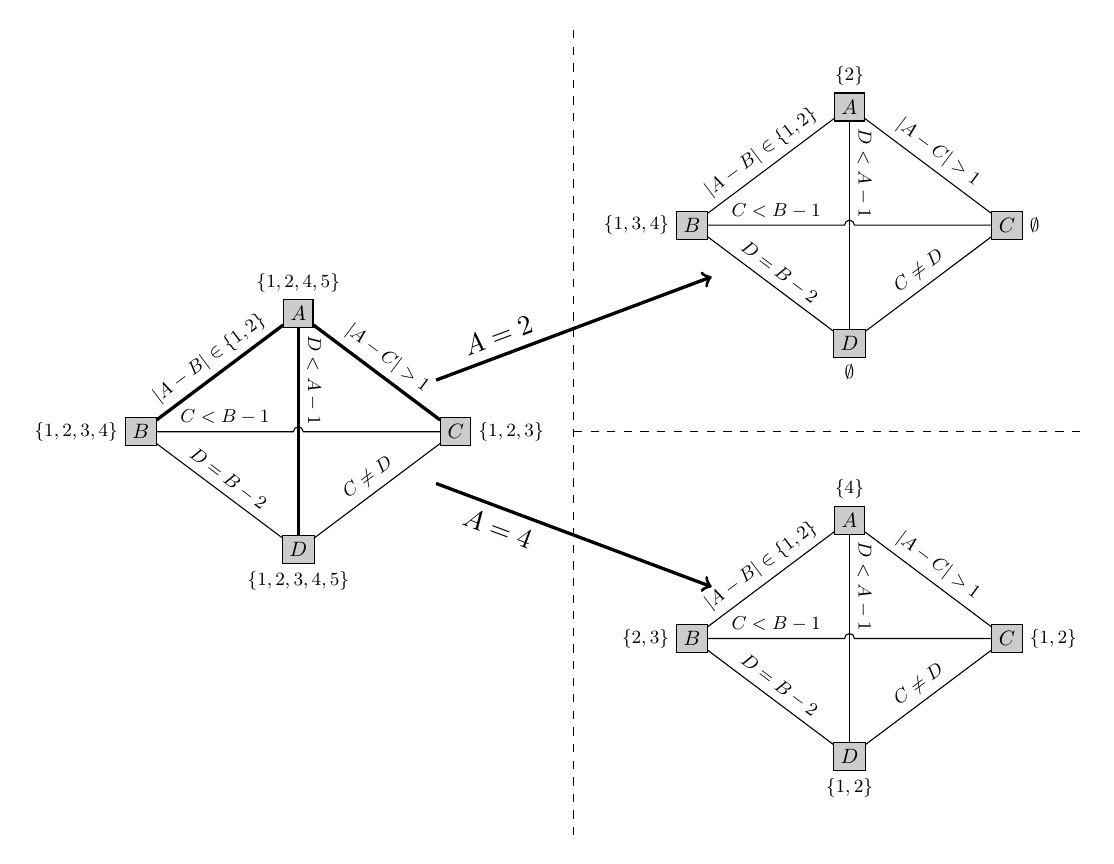
\begin{tikzpicture}[vari/.style={scale=0.75,fill=black!20,rectangle,draw=black}]
\def\dx{2};
\def\dy{1.5};
\def\r{0.0625};
\draw[dashed] (0,-2.75*\dy-1) -- (0,2.75*\dy+1);
\draw[dashed] (0,0) -- (2.75*\dx+1,0);
\begin{scope}[xshift=-1.75*\dx cm]
\node[vari] (A) at (0,\dy) {$A$};
\node[vari] (B) at (-\dx,0) {$B$};
\node[vari] (C) at (\dx,0) {$C$};
\node[vari] (D) at (0,-\dy) {$D$};
\node[scale=0.75,anchor=south] (DA) at (A.north) {\small{$\left\{1,2,4,5\right\}$}};
\node[scale=0.75,anchor=east] (DB) at (B.west) {\small{$\left\{1,2,3,4\right\}$}};
\node[scale=0.75,anchor=west] (DC) at (C.east) {\small{$\left\{1,2,3\right\}$}};
\node[scale=0.75,anchor=north] (DD) at (D.south) {\small{$\left\{1,2,3,4,5\right\}$}};
\draw[very thick] (A) to node[scale=0.75,midway,sloped,above]{\small{$\left|A-B\right|\in\left\{1,2\right\}$}} (B);
\draw[very thick] (A) to node[scale=0.75,midway,sloped,above]{\small{$\left|A-C\right|>1$}} (C);
\draw[very thick] (A) to node[scale=0.75,midway,sloped,above]{\small{$D<A-1$}} (0,0) -- (D);
\draw (B) to node[scale=0.75,midway,sloped,above]{\small{$C<B-1$}} (-\r,0) arc (180:0:\r) -- (C);
\draw (B) to node[scale=0.75,midway,sloped,above]{\small{$D=B-2$}} (D);
\draw (C) to node[scale=0.75,midway,sloped,above]{\small{$C\neq D$}} (D);
\end{scope}
\begin{scope}[xshift=1.75*\dx cm, yshift=1.75*\dy cm]
\node[vari] (A) at (0,\dy) {$A$};
\node[vari] (B) at (-\dx,0) {$B$};
\node[vari] (C) at (\dx,0) {$C$};
\node[vari] (D) at (0,-\dy) {$D$};
\node[scale=0.75,anchor=south] (DA) at (A.north) {\small{$\left\{2\right\}$}};
\node[scale=0.75,anchor=east] (DB) at (B.west) {\small{$\left\{1,3,4\right\}$}};
\node[scale=0.75,anchor=west] (DC) at (C.east) {\small{$\emptyset$}};
\node[scale=0.75,anchor=north] (DD) at (D.south) {\small{$\emptyset$}};
\draw (A) to node[scale=0.75,midway,sloped,above]{\small{$\left|A-B\right|\in\left\{1,2\right\}$}} (B);
\draw (A) to node[scale=0.75,midway,sloped,above]{\small{$\left|A-C\right|>1$}} (C);
\draw (A) to node[scale=0.75,midway,sloped,above]{\small{$D<A-1$}} (0,0) -- (D);
\draw (B) to node[scale=0.75,midway,sloped,above]{\small{$C<B-1$}} (-\r,0) arc (180:0:\r) -- (C);
\draw (B) to node[scale=0.75,midway,sloped,above]{\small{$D=B-2$}} (D);
\draw (C) to node[scale=0.75,midway,sloped,above]{\small{$C\neq D$}} (D);
\end{scope}
\begin{scope}[xshift=1.75*\dx cm, yshift=-1.75*\dy cm]
\node[vari] (A) at (0,\dy) {$A$};
\node[vari] (B) at (-\dx,0) {$B$};
\node[vari] (C) at (\dx,0) {$C$};
\node[vari] (D) at (0,-\dy) {$D$};
\node[scale=0.75,anchor=south] (DA) at (A.north) {\small{$\left\{4\right\}$}};
\node[scale=0.75,anchor=east] (DB) at (B.west) {\small{$\left\{2,3\right\}$}};
\node[scale=0.75,anchor=west] (DC) at (C.east) {\small{$\left\{1,2\right\}$}};
\node[scale=0.75,anchor=north] (DD) at (D.south) {\small{$\left\{1,2\right\}$}};
\draw (A) to node[scale=0.75,midway,sloped,above]{\small{$\left|A-B\right|\in\left\{1,2\right\}$}} (B);
\draw (A) to node[scale=0.75,midway,sloped,above]{\small{$\left|A-C\right|>1$}} (C);
\draw (A) to node[scale=0.75,midway,sloped,above]{\small{$D<A-1$}} (0,0) -- (D);
\draw (B) to node[scale=0.75,midway,sloped,above]{\small{$C<B-1$}} (-\r,0) arc (180:0:\r) -- (C);
\draw (B) to node[scale=0.75,midway,sloped,above]{\small{$D=B-2$}} (D);
\draw (C) to node[scale=0.75,midway,sloped,above]{\small{$C\neq D$}} (D);
\end{scope}
\draw[very thick,->] (-0.875*\dx,0.4375*\dy) to node[near start,above,sloped]{$A=2$} (0.875*\dx,1.3125*\dy);
\draw[very thick,->] (-0.875*\dx,-0.4375*\dy) to node[near start,below,sloped]{$A=4$} (0.875*\dx,-1.3125*\dy);
\end{tikzpicture}
\caption{Forward Check toegepast op het 4-Teachers probleem met $A=2$ en $A=4$.}
\label{fig:fourTeachersConstraintNetworkForwardCheck}
\end{figure}
\paragraph{Look Ahead Check}
Een andere techniek die de domeinen tracht te verkleinen is \termen{Look Ahead Check}. Hierbij ligt de focus niet op een variabele, zoals bij Forward Check, maar bij de constraints zelf. We itereren over iedere constraint $c\left(z_i,z_j\right)$ en kennen $z_i$ een bepaalde waarde toe. Indien voor om het even welke waarde van $z_j\in d_j$ de constraint blijft falen, is het duidelijk dat we de waarde van $z_i$ uit zijn domein $d_i$ mogen schrappen. Logischerwijs kunnen we dezelfde. Uiteraard werken we ook in de omgekeerde richting en zullen we zo ook het domein $d_j$ van $z_j$ zo kunnen verkleinen. Ook dit algoritme zal in het algemeen niet tot een consistente staat komen, de kettingreactie wordt immers opnieuw niet verwerkt. Een belangrijke eigenschap van dit algoritme is dat de volgorde waarin de constraints ge\"evalueerd worden, het resultaat kan be\"invloeden. Indien we bijvoorbeeld eerst het domein van een variabele verkleinen en daarna nog een andere constraint gerelateerd aan deze constraint onderzoeken, zullen we over het algemeen meer inconsistenties vinden. Formeel zeggen we dus dat voor een gegeven variabele $z_i$ we $a_{i\,k}$ kunnen verwijderen uit het domein indien geldt:
\begin{equation}
\exists c(z_i,z_j):\forall x\in d_j:\neg c\left(z_i=a_{i\,k},z_j=x\right)
\end{equation}
Of anders gezegd, er bestaat een constraint waarbij voor iedere waarde die de andere variabele aanneemt de constraint faalt.
\begin{leftbar}
We zullen dit concept illustreren door een Look Ahead Check uit te voeren op het 4-Teachers probleem. Als constraint nemen we $c\left(B,D\right)$. Zoals we op figuur \ref{fig:fourTeachersConstraintNetworkLookAheadCheck} zien, worden zowel de domeinen van $B$ als $D$ gereduceerd.
\end{leftbar}
\begin{figure}
\centering
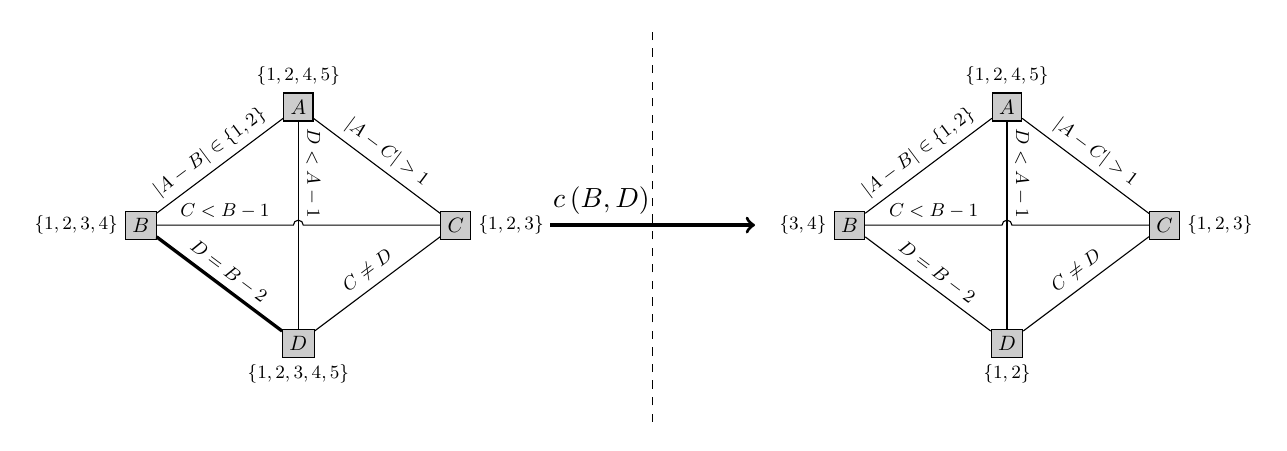
\begin{tikzpicture}[vari/.style={scale=0.75,fill=black!20,rectangle,draw=black}]
\def\dx{2};
\def\dy{1.5};
\def\r{0.0625};
\draw[dashed] (0,-\dy-1) -- (0,\dy+1);
\begin{scope}[xshift=-2.25*\dx cm]
\node[vari] (A) at (0,\dy) {$A$};
\node[vari] (B) at (-\dx,0) {$B$};
\node[vari] (C) at (\dx,0) {$C$};
\node[vari] (D) at (0,-\dy) {$D$};
\node[scale=0.75,anchor=south] (DA) at (A.north) {\small{$\left\{1,2,4,5\right\}$}};
\node[scale=0.75,anchor=east] (DB) at (B.west) {\small{$\left\{1,2,3,4\right\}$}};
\node[scale=0.75,anchor=west] (DC) at (C.east) {\small{$\left\{1,2,3\right\}$}};
\node[scale=0.75,anchor=north] (DD) at (D.south) {\small{$\left\{1,2,3,4,5\right\}$}};
\draw (A) to node[scale=0.75,midway,sloped,above]{\small{$\left|A-B\right|\in\left\{1,2\right\}$}} (B);
\draw (A) to node[scale=0.75,midway,sloped,above]{\small{$\left|A-C\right|>1$}} (C);
\draw (A) to node[scale=0.75,midway,sloped,above]{\small{$D<A-1$}} (0,0) -- (D);
\draw (B) to node[scale=0.75,midway,sloped,above]{\small{$C<B-1$}} (-\r,0) arc (180:0:\r) -- (C);
\draw[very thick] (B) to node[scale=0.75,midway,sloped,above]{\small{$D=B-2$}} (D);
\draw (C) to node[scale=0.75,midway,sloped,above]{\small{$C\neq D$}} (D);
\end{scope}
\begin{scope}[xshift=2.25*\dx cm]
\node[vari] (A) at (0,\dy) {$A$};
\node[vari] (B) at (-\dx,0) {$B$};
\node[vari] (C) at (\dx,0) {$C$};
\node[vari] (D) at (0,-\dy) {$D$};
\node[scale=0.75,anchor=south] (DA) at (A.north) {\small{$\left\{1,2,4,5\right\}$}};
\node[scale=0.75,anchor=east] (DB) at (B.west) {\small{$\left\{3,4\right\}$}};
\node[scale=0.75,anchor=west] (DC) at (C.east) {\small{$\left\{1,2,3\right\}$}};
\node[scale=0.75,anchor=north] (DD) at (D.south) {\small{$\left\{1,2\right\}$}};
\draw (A) to node[scale=0.75,midway,sloped,above]{\small{$\left|A-B\right|\in\left\{1,2\right\}$}} (B);
\draw (A) to node[scale=0.75,midway,sloped,above]{\small{$\left|A-C\right|>1$}} (C);
\draw (A) to node[scale=0.75,midway,sloped,above]{\small{$D<A-1$}} (0,0) -- (D);
\draw (B) to node[scale=0.75,midway,sloped,above]{\small{$C<B-1$}} (-\r,0) arc (180:0:\r) -- (C);
\draw (B) to node[scale=0.75,midway,sloped,above]{\small{$D=B-2$}} (D);
\draw (C) to node[scale=0.75,midway,sloped,above]{\small{$C\neq D$}} (D);
\end{scope}
\draw[very thick,->] (-0.65*\dx,0) to node[near start,above,sloped]{$c\left(B,D\right)$} (0.65*\dx,0);
\end{tikzpicture}
\caption{Look Ahead Check toegepast op het 4-Teachers probleem met $c\left(B,D\right)$.}
\label{fig:fourTeachersConstraintNetworkLookAheadCheck}
\end{figure}
\subsubsection{Arc Consistency Technieken}
Om de domeinen verder te verkleinen, en vervolgens tot een consistente staat te komen waarbij aan iedere constraint voldaan wordt, zijn een andere collectie algoritmen nodig, deze worden Arc Consistency Techniques of \termen{2-consistency} genoemd. Het principe is gebaseerd op herhalen van Weak Relaxation technieken tot een consistente staat bekomen wordt. We bespreken hieronder twee technieken.
\paragraph{AC1} Een eenvoudig algoritme dat ontwikkeld werd door Mackworth\footnote{Alan K. Mackworth} is \termen{AC1} of \termen{Arc Consistency 1}. Hierbij passen we het Look Ahead Algoritme toe tot geen enkel domein meer verkleind wordt. Het resultaat na het toepassen van dit algoritme, is een consistent netwerk van variabelen met een (verkleind) domein. Meestal bereiken we echter geen concrete oplossing. Bovendien is AC1 niet effic\"ent: Alle constraints worden gecontroleerd, ook degene die die niet gerelateerd zijn aan een variabele waar het domein verkleind is. In dat geval zal een extra evaluatie van de constraint, geen nieuwe inconsistenties opleveren, en dus nutteloos blijken.
\paragraph{AC3} Een oplossing voor dit effici\"entieprobleem werd ge\"implementeerd met \termen{Arc Consistency 3} of kortweg \termen{AC3}. Hierbij worden alle constraints in een wachtrij geplaatst. Vervolgens worden constraints in de wachtrij \'e\'en voor \'e\'en ge\"evalueerd. Indien deze constraint inconsistente waarden uit \'e\'en van de domeinen verwijdert, worden alle constraints die gerelateerd zijn aan de variabele met het gereduceerde domein in de wachtrij geplaatst. Het algoritme gaat door tot de wachtrij uiteindelijk leeg is. Dit is formeel beschreven in \algref{alg:arcConsistency3}.
\begin{algorithm}[htb]
\caption{Arc Consistency 3}
\label{alg:arcConsistency3}
\begin{algorithmic}[1]
\STATE $\queue\leftarrow\left\{c\left(z_i,z_j\right)|\forall i,j:i<j\right\}$
\WHILE{$\notempty{\queue}$}
\STATE$c\left(z_i,z_j\right)\leftarrow\dequeue{\queue}$
\STATE$d_{i}'\leftarrow\domain{z_i}$
\STATE$d_{j}'\leftarrow\domain{z_j}$
\STATE$\removeinconsistentvaluesof{z_i,z_j,c\left(z_i,z_j\right)}$
\IF{$\domain{z_i}\neq d_i'$}
\STATE$\enqueue{\queue,\left\{c\left(z_k,z_i\right)|\forall k:k<i\right\}\cup\left\{c\left(z_i,z_k\right)|\forall k:i<k\right\}}$
\ENDIF
\IF{$\domain{z_j}\neq d_j'$}
\STATE$\enqueue{\queue,\left\{c\left(z_j,z_k\right)|\forall k:j<k\right\}\cup\left\{c\left(z_k,z_j\right)|\forall k:k<j\right\}}$
\ENDIF
\ENDWHILE
\end{algorithmic}
\end{algorithm}
Dit algoritme geeft exact hetzelfde resultaat als AC1 maar in de meeste gevallen slechts de helft aan constraint-evaluaties. Opnieuw vinden we echter geen resultaat. Om dit probleem op te lossen, is een combinatie van backtracking algoritmen en relaxatie-algoritmen vereist. Deze worden nu behandeld in subsubsectie \ref{sss:hybridConstraintProcessing}.
\subsubsection{Hybrid Constraint Processing}
\label{sss:hybridConstraintProcessing}
Zoals reeds eerder vermeld zullen Arc Consistency technieken en Weak Relaxation algoritmen in het algemeen niet tot een concrete oplossing komen. Hiervoor is een combinatie van backtracking zoekmethoden en relaxatie nodig. Er zijn verschillende combinaties mogelijk, de meest relevante worden hieronder kort weergegeven.
\paragraph{Forward Checking}\termen{Forward Check\underline{ing}} (Niet te verwarren met Forward Check) is, zoals de naam al doet vermoeden, een combinatie van backtracking en Forward Check. Hierbij geeft het Chronologisch Backtrackingsalgoritme aan een bepaalde variabele een waarde, waarna Forward Check uitgevoerd wordt. Dit reduceert vervolgens de domeinen van de andere variabelen. Vervolgens zullen we een niveau lager in de boom zoeken, en een andere variabele een waarde toewijzen krijgt, en de lus opnieuw begint. Indien we tot situaties komen waarbij we een domein volledig leeghalen, kunnen we hieruit geen oplossing meer genereren, bijgevolg voeren we een backtracking uit. Belangrijk hierbij is op te merken dat de domeinen bij backtracking terug hun oorspronkelijke waarde moeten bekomen. En men dus niet eenvoudigweg de domeinen telkens mag verkleinen, deze hangen immers af van de gekozen waarden. Eventueel kan van het Dynamic Search Rearrangement Concept gebruik gemaakt worden.
\paragraph{Lookahead Checking}\termen{Lookahead Check\underline{ing}} (Niet te verwarren met Look Ahead Check) is, zoals de naam al doet vermoeden, een combinatie van backtracking en Lookahead Check. De werking van dit algoritme is behoorlijk analoog aan dat van Forward Checking, met als enig verschil dat Lookahead Check uitgevoerd wordt en niet Forward Checking. Ook hier kan een Dynamic Search Rearrangement nog extra tijdswinst opleveren.
\paragraph{Welk algoritme is het beste?}
Zowel Forward Checking als Lookahead Checking slagen er in de meeste gevallen in, tot een resultaat te komen binnen een redelijke tijd. Toch ligt de nadruk bij de twee algoritmen op verschillende plaatsen. Forward Checking zal over het algemeen minder consistency checks doen, met het gevolg dat de boom meer vertakkingen hebben. Anderzijds zal Lookahead Checking veel tijd investeren in het zoeken van inconsistenties, maar wint deze terug door minder grote bomen te genereren. Algemeen echter is Forward Checking beter, Lookahead Checking controleert immers alle constraints, ook wanneer er geen variabele aangepast is, en er dus geen verkleining van het domein mogelijk is. Indien een probleem echter veel (niet-triviale) constraints bevat kan Lookahead Checking beter presteren.
\subsection{$k$-consistency}
Naast $1$-consistency, en $2$-consistency, kan men dit principe uiteraard veralgemenen naar \termen{$k$-consistency}. In dat geval gelden er ook constraints, die uitspraken doen over de relatie van $k$ variabelen ten opzicht van elkaar. In OR-bomen wordt een dergelijke constraint ge\"evalueerd vanaf het moment dat alle variabelen die gerelateerd zijn aan de constraint een waarde toegewezen krijgen. Meestal komt dit er dus op neer dat de constraint zich op het niveau bevindt van de variabele met het hoogste index-cijfer. Ook Weak-Relaxation technieken kunnen veralgemeend worden om met deze situaties om te gaan, in het algemeen zal dit echter resulteren in een groot verlies van performantie. Dit omwille van twee redenen: de problemen zijn eenvoudigweg complexer en er is tot nu toe minder onderzoek in ge\"investeerd.
\subsection{Toepassingen en Alternatieven}
Constraint processing heeft toepassingen in allerhande industri\"ele takken van de samenleving gaande van het opstellen van uurroosters over het laden van trucks tot het programmeren van robotarmen. Een bekende taal om constraint systemen te beschrijven is Prolog\footnote{Programmation en Logique}.
\begin{leftbar}
We drukken het 4-Teachers probleem hieronder formeel uit in SWI-Prolog:
\begin{verbatim}
:- use_module(library(clpfd)).        %laad de constraint processing module in

fourTeachers([A,B,C,D]) :-
    Vars = [A,B,C,D],                 %variabelen initialiseren
    Vars ins 1..5,                    %domein specifieren
    A #\= 3,                          %c(A)
    B #\= 5,                          %c(B)
    C #=< 3,                          %c(C)
    abs(A-B) #>= 1, abs(A-B) #=< 2,   %c(A,B)
    abs(A-C) #> 1,                    %c(A,C)
    D #< A-1,                         %c(A,D)
    C #< B-1,                         %c(B,C)
    D #= B-2,                         %c(B,D)
    C #\= D,                          %c(C,D)
    label(Vars).                      %los het constraint probleem op.
\end{verbatim}
We kunnen dan vervolgens een query aanroepen in SWI-Prolog die ons het resultaat van de puzzel teruggeeft:
\begin{verbatim}
?- fourTeachers(S).
S = [5, 4, 1, 2].
\end{verbatim}
Indien we de laatste opdracht \verb+label/1+ weglaten dan wordt het constraint probleem niet opgelost. Dit vertelt ons echter iets meer over de werking van SWI-Prolog: Er wordt een Look Ahead Check uitgevoerd op het probleem, in de volgorde dat de constraints worden gedefinieerd. In dat geval wordt een reeks constraints als uitvoer geschreven die het probleem beschrijft inclusief de optimalisaties gegenereerd door Look Ahead Check:
\begin{verbatim}
?- fourTeachersNoLabel([A,B,C,D]).
A in 4..5,
_G3451+B#=A,
abs(A-C)#>=2,
abs(A-B)#>=1,
D in 1..2,
C#\=D,
D+2#=B,
C in 1..2,
C#=<B+ -2,
B in 3..4,
_G3451 in 0..2.
\end{verbatim}
\end{leftbar}
\paragraph{}
Alternatieven komen vooral uit de hoek van \termen{Linear Programming}. Dit zijn een reeks numerieke en algebra\"ische technieken die over het algemeen zeer effici\"ent werken voor linear constraints (Constraints waar alleen vermenigvuldigingen met constanten en optellingen in voorkomen), een voorbeeld hiervan is het ``Simplex Algoritme'', indien we echter niet-lineare constraints beschouwen is Constraint Processing de aangewezen methode, verder kan Constraint Processing ook overweg met niet numerieke data (zoals bijvoorbeeld tekst, lijsten,...).
